\documentclass[letterpaper]{article}
\usepackage{natbib,alifexi}
\usepackage[bordercolor=gray!20,backgroundcolor=blue!10,linecolor=blue,textsize=footnotesize,textwidth=0.8in]{todonotes}
\usepackage{hyperref}

\title{Implementation\\Playing FPS Games with Deep Reinforcement Learning}
\author{Titouan Christophe$^{1}$, Florentin Hennecker$^{2}$, Nikita Marchant$^{1}$ \and Bruno Rocha Pereira$^{1}$ \\
\mbox{}\\
$^1$Vrije Universiteit Brussel, Pleinlaan 2, 1050 Brussels, Belgium \\
$^2$Universit\'e Libre de Bruxelles, Boulevard du Triomphe - CP 212, 1050
Brussels, Belgium \\
\{nimarcha,brochape\}@vub.ac.be, fhenneck@ulb.ac.be, tichrist@vub.be}

\marginparwidth=0.5in
\newcommand\Tstrut{\rule{0pt}{2.6ex}}
\newcommand\Bstrut{\rule[-0.9ex]{0pt}{0pt}}


\begin{document}
\maketitle

\begin{abstract}
\end{abstract}

\section{Introduction}
Deep Reinforcement learning has brought in the past solutions to automating and
learning typical human-computer interactions. \todo{refs!}
However, most of the previous applications of Deep Q-Networks assume a full
knowledge of their environment. The application of those traditional DQN is
thus limited in the case of playing FPS\footnote{First Person Shooter} games,
where the field of vision of the player is limited. Deep recurrent networks
were proposed to solve this problem \citep{Hausknecht2015} applied to Atari
game. This paper applies techniques used for 2D games and extends them for use
on a 3D game named DOOM.
In order to plug our work to the DOOM game, we are using the Vizdoom API
\citep{Kempka2016} that provides an easy use of the game controls as well as
knowledge about the current state of the game.
The agents will be playing in a setup of deathmatch. This means that they play
in a level that requires to have the maximum amount of kills and the minimum
amount of deaths, which is called best k/d ratio.
In this paper, we are implementing the techniques described in
\citep{Lample2016}.
\todo{say that we're only playing basic}

\section{Methods}

\subsection{Background}
\subsubsection{Deep Q-Networks}
Many reinforcement learning problems have a very high-dimensional space-state
in which each dimension on its own bears very little information. Approximating
a state-action $Q$ function over all possible states and actions becomes quickly
intractable. However, deep neural networks have an outstanding capability to
encode high-dimensional states into a lower-dimensional hidden state; moreover,
they are also known for their function approximation capabilities
\citep{Hornik1991}. Deep Q-Learning \citep{Mnih2015} is a major breakthrough
showing that neural networks can learn to play Atari games.

In the context of a Deep Q-Network (DQN), an agent tries to learn
$Q(s_t,a_t)$ which represents an
estimation of how valuable an action $a_t$ is in a state $s_t$. In order to
find $Q^*$, the optimal $Q$-function, DQNs use a neural network
parametrized by $\theta$, which represents the weights of the neural network
and gives an approximation called $Q_\theta$ further in this paper. Their goal
is to find the optimal and real $Q$-function $Q^*$ which is verifies the Bellman
optimality equation:
$$ Q^*(s,a) = E\{r + \gamma \max_{a'}Q^*(s',a')|s,a\} $$
With $r$ being the reward of playing $a$ in a state $s$, $\gamma\in [0,1]$ the
discount factor and $(s',a')$ being the next state and its associated action

This gives, since $Q_{\theta} \approx Q^*(s,a)$ the loss function below:
$$ L_\theta(\theta_t) = E_{s,a,r,s'}\{(r +\gamma \max_{a'}Q_\theta(\theta_t)(s' , a' )-Q_{\theta_t}(s,a))^2\}$$

This loss is computed on uniformly sampled game transitions stored in a
replay memory instead of the previously played transition to reduce correlation
between samples.


\subsubsection{Deep Recurrent Q-Networks}
One of the issues posed by the model described above is that it assumes that the
environment is fully observable. However in the case of DOOM, we only get a
partial
observation of the environment, limited by the field of vision of the main
character. Previous ways of solving that issue have been to feed a sequence of
frames to the DQN as a history.
A potentially better way to solve the history issue is to use a Deep Recurrent
Q-Network, as described in \citep{Hausknecht2015}. A DRQN
estimates $Q(s_t,h_{t-1},a_t)$ instead of the regular $Q(s_t,a_t)$. The
parameter $h_{t-1}$ represents the hidden state of the agent at the previous
transition. In our case, we will use an LSTM to generate a new output and a new
hidden state given an input and the previous hidden state.
\todo{Adapter à notre archi}

\subsection{Model details}
Our neural network is the same as the one presented in \citep{Lample2016},
with one addition.
It is composed of two convolutional layers followed by three separate
sub-networks. One of these sub-networks is used in a supervised manner to
predict various game features (see below), the second is a standard
DRQN network while the last is a standard DQN output. The network is trained
with or without the game features and with either the DRQN or the DQN output.
The hidden size of the LSTM was set to 300 units.

\begin{figure}[h]
  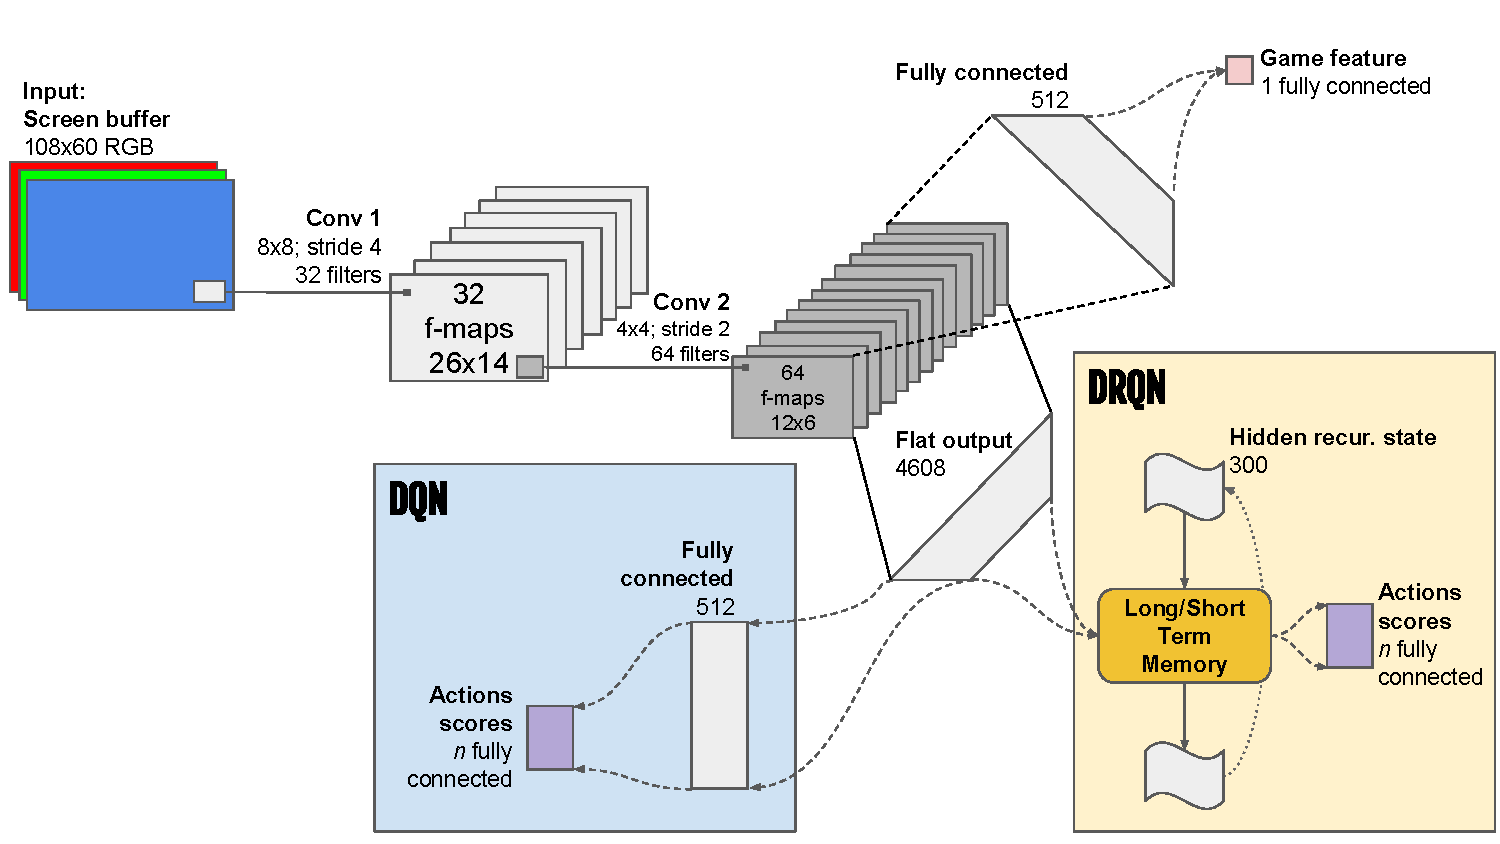
\includegraphics[width=\textwidth]{DRQNSchema.pdf}
  \caption{\label{fig:drqn-schema} Our network and its variations}
\end{figure}

\subsubsection{Game Features} As described in the paper \citep{Lample2016},
agents not using the game features were unable to accurately detect enemies and
were thus randomly shooting around hoping that those shots would reach their
targets. In order to make up for a lack of efficiency, we used custom made game
features to train the agent in a supervised setup jointly with the Q-learning
setup to tell the agent if enemies were in his field of vision.  The
\texttt{Label buffer} provided by the Vizdoom API  was used to fetch all the
entities present in the vision frustum. However, entities hidden by other scene
elements, typically walls, were also parts of that buffer. We then used the map
characteristics in order to to check if an entity was visible or not. Even
though this information can't be used during testing phase, it was used during
the training of the agents to improve their accuracy. We also created a game
feature estimating the lateral position of an enemy against a wall in a much
simpler DOOM map.

\subsubsection{Frame Skip}
To reduce the computational complexity, it is common to use the skip-frame
technique. With this technique, the agent receives a input frame every $k + 1$
game frames, where $k$ is the number of of frames skipped. During those
skipped frames, the last action of the agent is repeated automatically.
We used a value of $k=4$ because it is a good trade-off between
computing performance and agent accuracy \citep{Kempka2016}.


\subsubsection{Sequential Updates}
When training an LSTM, one feeds sequences of data for which the LSTM will
predict one output per time step. However, the LSTM will zero its hidden state
before the start of each sequence, and it will take several time steps for the
hidden state to initialise. Hence, the outputs for the first time steps might
be erroneous since their previous hidden state was not fully initialised. 
To solve this, we discard the first time steps outputs when computing the loss,
as explained in \citep{Lample2016}.

\subsubsection{Hyperparameters}
Analogously to \cite{Mnih2015} and \cite{Lample2016}, we use a replay memory
size of $1000000$ frames. The sequence length of
the training samples was set to 8, but only the last 4 outputs were accounted
in the loss.
Each frame consists of a 8 bit per color \texttt{RGB} buffer of dimension
$60 * 108$\footnote{As VizDoom does not support natively this resolution, we
used the $200 * 125$ resolution and downsampled it before feeding it to the
agent.}.
In the bootstrapping phase, our agent only plays random actions drawn from the
set \texttt{TURN\_LEFT, MOVE\_LEFT, MOVE\_FORWARD, JUMP, MOVE\_RIGHT}. We do
not add the \texttt{TURN\_RIGHT} and \texttt{MOVE\_BACKWARD} actions, because
a uniformly random sample of all these actions would lead the agent to stay
at the same place and face approximately the same direction all the time. This
bootstrapping phase is used to populate the replay memory.

We used the RMSProp\todo{ref slides} algorithm with a learning rate of 0.001.

\subsubsection{Dropout}
Dropout \citep{Srivastava2014} was added to the fully connected layers, with
a probability of keeping each unit of 75\% at training time.

\subsection{Action phase}
As opposed to the paper \citep{Lample2016} which uses a navigation phase as
well as an action phase, we decided to only focus on the action phase. The
navigation phase is the phase where the agent focuses on exploring the map to
collect items and find enemies. We indeed dropped that step to immediately
concentrate our efforts on the action phase, which consists in shooting at
enemies when they are detected. This so-called action phase will of course
take place after a training phase during which the agent learns how to interact
properly with the game.

\subsection{Implementation}
We implemented the model using Python 3 and Tensorflow \citep{tensorflow}.
It is available publicly on Github
\footnote{\url{https://github.com/fhennecker/deepdoom}}.



\section{Results}
\begin{table}[h]
\centering
\begin{tabular}{cc}
\multicolumn{2}{c}{Test Setup}                         \Tstrut\\ \hline
\multicolumn{1}{c|}{CPU} & Intel i7-6800K 3.4 GHz      \Tstrut\\
\multicolumn{1}{c|}{GPU} & Nvidia GeForce GTX 1080 8Go \Tstrut\\
\multicolumn{1}{c|}{RAM} & 32 Go DDR4                      \Tstrut
\end{tabular}
\caption{Test setup hardware specification}
\label{tab:specs}
\end{table}

The training phase as well as the action phase were run on a high-end machine
of which specifications are displayed in Table \ref{tab:specs}.

\section{Discussion}


\footnotesize
\bibliographystyle{apalike}
\bibliography{report}


\end{document}
